\documentclass[a4paper, 12pt]{article}
\usepackage[utf8]{inputenc}
\usepackage{mathptmx}
\usepackage[T1]{fontenc}
\usepackage[utf8]{inputenc}
\usepackage[style=apa,backend=biber]{biblatex}
\addbibresource{literature.bib}
\usepackage{listingsutf8}
\usepackage{graphicx}
\usepackage{longtable}
\usepackage{booktabs}
\usepackage{listings}
\usepackage{xcolor}
\usepackage{enumitem}
\usepackage{pdfpages}

\definecolor{codegreen}{rgb}{0,0.6,0}
\definecolor{codegray}{rgb}{0.5,0.5,0.5}
\definecolor{codepurple}{rgb}{0.58,0,0.82}
\definecolor{backcolour}{rgb}{0.95,0.95,0.92}

\lstset{
    backgroundcolor=\color{gray!10},   
    commentstyle=\color{codegreen},
    keywordstyle=\color{magenta},
    numberstyle=\tiny\color{codegray},
    stringstyle=\color{codepurple},
    basicstyle=\ttfamily\footnotesize,
    breakatwhitespace=false,         
    breaklines=true,                 
    captionpos=b,                    
    keepspaces=true,                 
    numbers=left,                    
    numbersep=5pt,                  
    showspaces=false,                
    showstringspaces=false,
    showtabs=false,                  
    tabsize=2,
    inputencoding=utf8,
    extendedchars=false,
    escapeinside={\%*}{*)},
}
\usepackage{hyperref}
\hypersetup{
	pdftitle={When Blocks Build Societies: Multi-Agent Systems in Minecraft},
    pdfauthor={Jan-Philipp Kiel},
	pdfnewwindow=true,
	% colorlinks=false,
	% linktoc=page,     % nur seitennummern verlinkt
	linktoc=all, % sections und subsections verlinkt
	% linkcolor=black,
	% urlcolor=black,
	% bookmarks=true,
	% citecolor=black
}
\usepackage[labelfont=bf]{caption}
\captionsetup[table]{justification=raggedright, singlelinecheck=false, labelfont=normalfont}
\usepackage{float}

% set margins for double-sided printing
\usepackage[left=4cm, right=2.5cm, top=2.5cm, bottom=2.5cm]{geometry} 
\usepackage{setspace}
% \onehalfspacing
% set header
\usepackage{fancyhdr}
\pagestyle{fancy}
\fancyhead{}
\fancyfoot{}
\fancyhead[L]{When Blocks Build Societies: Multi-Agent Systems in Minecraft}
\fancyfoot[R]{\thepage}
\fancypagestyle{plain}[fancy]{} % use fancy style for TOC
\setlength{\headheight}{15pt}
\usepackage{indentfirst} % indent first paragraph after section heading
\setlength{\parindent}{3em}

% Section heading font sizes
\usepackage{titlesec}
\titleformat{\section}{\normalfont\bfseries\fontsize{14}{16}\selectfont}{\thesection}{1em}{}
\titleformat{\subsection}{\normalfont\bfseries\fontsize{13}{15}\selectfont}{\thesubsection}{1em}{}
\titleformat{\subsubsection}{\normalfont\bfseries\fontsize{12}{14}\selectfont}{\thesubsubsection}{1em}{}
\titlespacing*{\section}{0pt}{1em}{0em}
\titlespacing*{\subsection}{0pt}{1em}{0em}
\titlespacing*{\subsubsection}{0pt}{1em}{0em}

% Table of Contents formatting
\usepackage{tocloft}
\renewcommand{\contentsname}{Table of Contents}
\renewcommand{\cfttoctitlefont}{\fontsize{14}{16}\selectfont\bfseries}
\renewcommand{\cftsecleader}{\cftdotfill{\cftdotsep}}
\renewcommand{\cftdotsep}{0.5}
\renewcommand{\cftsecnumwidth}{2em}
\renewcommand{\cftsubsecnumwidth}{3em}
\renewcommand{\cftsubsubsecnumwidth}{4em}
\renewcommand{\cftsubsecindent}{4em}
\renewcommand{\cftsubsubsecindent}{7em}
% Remove extra space before page numbers in TOC
\renewcommand{\cftsecafterpnum}{\hspace{0pt}}
\renewcommand{\cftsubsecafterpnum}{\hspace{0pt}}
\renewcommand{\cftsubsubsecafterpnum}{\hspace{0pt}}
\renewcommand{\cftsecfont}{\normalfont}
\renewcommand{\cftsecpagefont}{\normalfont}
\renewcommand{\cftbeforesecskip}{0pt}
\renewcommand{\cftsecindent}{0pt}
\renewcommand{\cftbeforesubsecskip}{0pt}
% Increase indentation for subsections and subsubsections in TOC
\renewcommand{\cftsubsecindent}{4em}
\renewcommand{\cftsubsecnumwidth}{4em}
\renewcommand{\cftsubsubsecindent}{5em} 
\renewcommand{\cftsubsubsecnumwidth}{3em}

% List formatting and bullet size
\renewcommand{\labelitemi}{\normalsize$\bullet$}
\setlist[itemize]{leftmargin=*, labelsep=1em}
\setlist[enumerate]{leftmargin=*, labelsep=1em}

% set APA citation style
% \usepackage{apacite}
\usepackage[nottoc]{tocbibind}

% Version Watermark
\usepackage{gitinfo2} % Gitinfo
\newcommand{\lastChange}{\gitCommitterIsoDate}
\usepackage{background}
\backgroundsetup{
	contents=\Large{\texttt{\MakeUppercase{\gitBranch}-\gitDescribe{ @ }\lastChange}},
	color=red,
	placement=center,
	angle=90,
	opacity=1,
	vshift=9cm,
	scale=1
}

\begin{document}

\setstretch{1.5}
\pagenumbering{Roman}

\begin{titlepage}
    \begin{center}
        \vspace*{\fill}
        \vspace*{-2cm}
        \large
        {\bfseries{When Blocks Build Societies}}\\
        Multi-Agent Systems in Minecraft\\

        \vspace{1cm}

        Jan-Philipp Kiel\\
        University of Cologne

        \vspace{1cm}

        Advanced Seminar\\
        Information Systems and Digital Technology\\
        Prof. Dr. Stefan Seidel

        \vspace{1cm}

        \today
        \vspace*{\fill}
    \end{center}
\end{titlepage}

\clearpage
% Table of Contents self-reference
% \addcontentsline{toc}{section}{Table of Contents}
\tableofcontents
\clearpage
% \listoffigures
% \clearpage
% \listoftables
% \clearpage

\pagenumbering{arabic}


%%%%%%%%%%%%%%%%%%%%%%%%%%%%%%%%%%%%%%%%%%%%%%%%%%%%%%%%%%%%%
%MAIN PART
%%%%%%%%%%%%%%%%%%%%%%%%%%%%%%%%%%%%%%%%%%%%%%%%%%%%%%%%%%%%%

\section{Introduction}

Multi-agent systems (MAS) are a key frontier in artificial intelligence (AI) research, offering insights into how autonomous entities can collaborate, compete, and coexist within shared environments \autocite{Leeuwen2021, Shu2024}. These systems enable the study of complex emergent behaviors and collective intelligence that extend beyond the capabilities of single agents \autocite{Leeuwen2021, Shu2024}. As AI continues to advance, understanding the principles that govern effective multi-agent collaboration becomes increasingly vital for applications ranging from robotic teams to virtual assistants \autocite{Leeuwen2021}.

Despite advances in MAS, there is limited understanding of how different collaborative frameworks---task-oriented versus socially-oriented---impact sustainable collaboration in complex virtual environments such as Minecraft. This paper addresses the need to compare these approaches to inform future design of collaborative MAS. The scope of this research is limited to Minecraft-based MAS. While potential parallels to other domains are discussed, all findings and design principles are grounded in the Minecraft context.

Minecraft, with its open-world sandbox, procedurally generated environments, and flexible crafting, make it an ideal platform for multi-agent research \autocite{Fan2022}. Its block-based world allows for precise control while still presenting meaningful challenges in navigation, resource gathering, construction, and social interaction \autocite{Zhao2024}.

Most MAS research in Minecraft has focused on specific task completion, such as navigation or building predefined structures. However, a  significant gap exists between these narrowly defined task-oriented systems and more complex, socially-oriented agent societies \autocite{Shu2024, Qiu2024}. Bridging this gap requires new approaches to agent architecture, communication protocols, and coordination mechanisms that can support sustainable collaboration over extended periods.

Two recent research initiatives have made significant progress in addressing different aspects of this challenge: Project Sid and TeamCraft. Project Sid, introduced in 2024, explores large-scale simulations of 10-1000+ AI agents, focusing on how these agents develop specialized roles, adhere to collective rules, and engage in cultural transmission within a civilization-inspired framework \autocite{Altera2024}. In contrast, TeamCraft provides a multi-modal multi-agent benchmark featuring 55,000 task variants designed to test various aspects of agent collaboration through structured prompts and demonstrations \autocite{Long2024}.

This paper addresses the research question: \textit{How do different collaborative frameworks in Minecraft address the challenge of sustainable multi-agent collaboration within virtual environments?} By comparing these approaches, we aim to identify design principles that can inform the development of more robust and adaptable collaborative AI systems within virtual environments.

The paper is structured as follows: First, we review background literature on MAS, Minecraft as a research platform, and approaches to approaches to agent collaboration. Next, we detail our methodology, including case study selection criteria and analytical framework. We then analyze Project Sid and TeamCraft individually before conducting a comparative analysis across organizational structures, communication patterns, learning mechanisms, and sustainability. Finally, we discuss theoretical implications, explore speculative practical applications in other domains, and conclude with directions for future research.

\section{Background and Related Work}

To ensure conceptual clarity, this paper adopts the following definitions: An \textit{agent} is an entity perceiving and acting on its environment \autocite{Russell2009}; \textit{artificial intelligence (AI)} is the study of agents maximizing cumulative reward \autocite{Russell2009}; a \textit{multi-agent system (MAS)} consists of multiple interacting agents whose collective behavior emerges from their interactions \autocite{Wooldridge2009}; and \textit{collaboration} refers to agents working together to achieve shared goals, requiring coordination and communication \autocite{Panait2005}.

\subsection{Multi-Agent Systems in Virtual Environments}

MAS represent a paradigm in AI research where multiple autonomous agents interact within a shared environment to achieve individual or collective goals \autocite{Leeuwen2021, Shu2024}. The field has evolved significantly from early distributed AI research in the 1980s to contemporary approaches leveraging deep learning and reinforcement learning \autocite{Leeuwen2021, Shu2024}. Modern MAS research encompasses diverse architectures ranging from fully cooperative to competitive and mixed-motive scenarios, with applications spanning robotics, logistics, gaming, and social simulation \autocite{Leeuwen2021, Shu2024}.

Virtual environments offer particularly valuable platforms for multi-agent research due to their controlled conditions, cost-effectiveness, and ability to simulate complex scenarios that would be impractical or impossible in physical settings \autocite{Shu2024, Lhaksmana2018}. These environments provide a ``consequence-free'' space to test agent behaviors that might be risky or expensive in real-world settings, while still capturing essential dynamics of multi-agent interaction \autocite{Shu2024, Lhaksmana2018}. Additionally, virtual environments allow researchers to precisely control experimental conditions and collect comprehensive data about agent behaviors and interactions \autocite{Shu2024, Lhaksmana2018}.

Multi-agent architectures can be broadly categorized as centralized or decentralized, with various hybrid approaches emerging to leverage the advantages of both \autocite{Leeuwen2021}. Centralized approaches maintain a global view of the environment and coordinate agent actions through a central controller, offering optimal decision-making at the cost of scalability and robustness \autocite{Leeuwen2021}. Decentralized approaches distribute decision-making among individual agents, providing resilience and scalability at the expense of potentially suboptimal coordination \autocite{Leeuwen2021}. Communication models within these architectures range from direct message passing to stigmergic coordination through environmental modifications \autocite{Leeuwen2021}.

Recent advances in multi-agent collaboration have been driven by developments in large language models (LLMs) and deep reinforcement learning \autocite{Shu2024, Qiu2024}. LLMs have enhanced agents' ability to understand complex instructions and generate contextually appropriate responses, while reinforcement learning techniques have improved adaptation to dynamic environments and coordination among heterogeneous agents \autocite{Chen2024}. These advances have expanded the scope of multi-agent research to include emergent communication protocols, collective intelligence, and social learning \autocite{Shu2024, Qiu2024, Chen2024}.

\subsection{Minecraft as a Research Platform}

Minecraft offers a uniquely suitable platform for AI research due to its procedurally generated worlds, comprehensive crafting system, and physics simulation that strikes a balance between realism and abstraction \autocite{Fan2022}. The game's block-based structure provides a discretized state space that is more computationally tractable than continuous environments while still offering sufficient complexity to model interesting real-world problems \autocite{Fan2022}. Furthermore, its open-world nature allows for a wide range of tasks, from simple navigation to complex collaborative construction projects \autocite{Fan2022}.

Previous AI research in Minecraft has explored diverse challenges, including single-agent task completion, navigation in procedurally generated landscapes, and creative building \autocite{Zhao2024, Wang2025}. The MineDojo framework, for instance, provides thousands of diverse open-ended tasks and an internet-scale knowledge base with Minecraft videos, tutorials, and forum discussions to facilitate agent learning \autocite{Fan2022}. Similarly, JARVIS-1 demonstrates how multimodal language models can perceive visual observations and textual instructions to generate sophisticated plans and perform embodied control in Minecraft \autocite{Wang2025}.

The Minecraft environment presents unique challenges for AI research, including a large state space, partial observability, and the need for long-horizon planning \autocite{Fan2022, Wang2025}. Agents must reason about objects that may be out of view, plan sequences of actions that may take hundreds or thousands of steps to complete, and adapt to unexpected environmental changes \autocite{Fan2022, Wang2025}. These challenges make Minecraft particularly valuable for testing the limits of current AI approaches and driving innovations in planning, perception, and learning algorithms \autocite{Fan2022, Wang2025}.

Beyond technical challenges, Minecraft enables social interaction and emergent behaviors that are difficult to study in more constrained environments \autocite{Altera2024, Yu2024}. The MineLand simulator, for example, introduces features like limited multimodal senses and physical needs to create more ecologically valid social interactions among large groups of agents \autocite{Yu2024}. This capability for modeling complex social dynamics makes Minecraft an ideal test bed for studying how artificial societies might form, evolve, and sustain themselves over time \autocite{Altera2024, Yu2024}.

\subsection{Approaches to Agent Collaboration}

Agent collaboration approaches typically fall into two broad categories: task-oriented collaboration, which focuses on completing specific objectives, and social-oriented collaboration, which emphasizes emergent social structures and norms \autocite{Shu2024, Qiu2024}. Task-oriented approaches typically define explicit goals, roles, and protocols for interaction, prioritizing efficiency and measurable outcomes \autocite{Shu2024, Qiu2024}. Social-oriented approaches, in contrast, allow organizational structures and behavioral norms to emerge through repeated interactions, often leading to more adaptable but less predictable collaborative behaviors \autocite{Shu2024, Qiu2024}.

Coordination mechanisms in MAS include role assignment, task allocation, and conflict resolution strategies \autocite{Dong2024, Shu2024}. Role-based approaches assign specific responsibilities to agents based on their capabilities or position within an organizational structure \autocite{Dong2024, Shu2024}. Task allocation methods distribute work among agents to optimize resource utilization and minimize conflicts \autocite{Dong2024, Shu2024}. These mechanisms may be static (predetermined) or dynamic (adapting to changing conditions), with varying degrees of centralization in decision-making authority \autocite{Dong2024, Shu2024}.

Communication strategies play a crucial role in effective collaboration, ranging from direct communication through message passing to indirect communication through environmental modifications \autocite{Shu2024,Qiu2024}. Direct communication allows for precise information sharing but requires protocols for when, what, and how to communicate \autocite{Shu2024, Qiu2024}. Indirect communication (stigmergy) relies on agents observing and responding to changes in the shared environment, often leading to emergent coordination patterns \autocite{Shu2024, Qiu2024}. The choice of communication strategy significantly impacts a system's scalability, robustness, and adaptability to novel situations \autocite{Shu2024, Qiu2024}.

Evaluation metrics for successful collaboration include task completion rates, resource efficiency, adaptability to changing conditions, and robustness to agent failures \autocite{Shu2024,Qiu2024, Chen2024}. Task-oriented systems typically prioritize metrics related to goal achievement and efficiency, such as time-to-completion and resource consumption \autocite{Shu2024, Qiu2024, Chen2024}. Social-oriented systems may emphasize metrics related to sustainability and resilience, such as the stability of social structures and adaptability to unexpected challenges \autocite{Shu2024, Qiu2024, Chen2024}. These different evaluation priorities reflect fundamental differences in how collaboration is conceptualized across approaches \autocite{Shu2024, Qiu2024, Chen2024}.

\section{Methodology}

This study uses a comparative case study approach to analyze multi-agent collaboration in Minecraft, following established guidelines from \textcite{Yin2018} and \textcite{Eisenhardt1989}. The process included: (1) identifying and screening candidate systems using explicit inclusion and exclusion criteria; (2) conducting a literature search across major academic databases; (3) applying a structured analytical framework to compare selected cases; and (4) documenting the use of generative AI tools, including ethical considerations and verification procedures. This ensures transparency, replicability, and systematic analysis \autocite{Yin2018, Eisenhardt1989}.

Project Sid and TeamCraft were selected as recent, well-documented, and conceptually contrasting case studies. Other systems were excluded due to overlap or insufficient distinctiveness. The analytical framework compares organizational structure, communication and coordination, learning and adaptation, and sustainability and scalability.

Generative AI tools supported literature review, synthesis, and drafting. All AI-generated content was reviewed and verified by the author. Limitations include potential selection bias, incomplete literature coverage, and risks of AI-generated inaccuracies. These were mitigated by explicit criteria, multi-database searches, and systematic verification against original sources.

\subsection{Case Study Selection}

Project Sid and TeamCraft were selected as the most methodologically robust and conceptually contrasting case studies of multi-agent collaboration in Minecraft. Selection followed criteria outlined by \textcite{Yin2018} and \textcite{Eisenhardt1989} and was based on recency, documentation quality, and clear contrast in collaborative paradigms. Other case studies were excluded for reasons such as overlap in paradigm, lack of focus on multi-agent collaboration, or insufficient distinctiveness. A detailed overview of all candidate case studies and selection rationale is provided in Table~\ref{tab:casestudycomparison}.

\subsection{Literature Search and Screening}

The literature search for candidate case studies was conducted between June and July 2025 using major academic databases including Google Scholar, Semantic Scholar, and arXiv. Search keywords included combinations of ``multi-agent systems'', ``Minecraft'', ``collaboration'', ``benchmark'', and ``emergent behavior''. Initial results were screened for relevance based on title and abstract. Full texts were reviewed for systems that focused on multi-agent collaboration in Minecraft environments. Generative AI tools were used to assist in the screening and review of identified papers, enabling efficient processing and synthesis of the literature. Additionally, conversational learning with AI was used to quickly understand key concepts and frameworks; the conversation histories are referenced in the appendix (see Appendix~\ref{appendix:aiconversationhistory}).

\subsection{Analytical Framework}

The comparative analysis employs a structured framework examining four key dimensions: (1) Organizational structure, (2) Communication and coordination, (3) Learning and adaptation, and (4) Sustainability and scalability. Each dimension is analyzed through the lens of established MAS literature and organizational theory, providing a systematic basis for comparison \autocite{Lhaksmana2018, Chen2024}.

Organizational structure is relevant because the way agents are organized---whether through emergent hierarchies or predefined roles---directly influences the system's ability to support sustainable collaboration and adapt to changing environments \autocite{Lhaksmana2018, Chen2024}. Communication and coordination are central to effective multi-agent collaboration, as the mechanisms for information exchange and joint action determine how well agents can work together to achieve shared goals \autocite{Shu2024, Qiu2024}. Learning and adaptation are crucial for long-term sustainability, enabling agents to improve their behaviors and strategies in response to new challenges and evolving contexts \autocite{Shu2024, Chen2024}. Sustainability and scalability address the research question by evaluating whether collaborative frameworks can maintain performance and resilience as the number of agents and complexity of tasks increase, which is essential for robust multi-agent societies in virtual environments like Minecraft \autocite{Shu2024, Chen2024}.

Organizational structure is analyzed through the lens of hierarchy (the levels of authority and decision-making in the system), role specialization (how agents develop specialized functions), and adaptability (how the organization responds to changing conditions) \autocite{Lhaksmana2018, Chen2024}. Project Sid's emergent hierarchies are contrasted with TeamCraft's task-oriented organization to understand how different structural approaches affect collaborative outcomes. This analysis draws on organizational theory concepts such as centralization, formalization, and departmentalization to characterize the systems' organizational features \autocite{Lhaksmana2018, Chen2024}.

Agent autonomy and communication patterns are evaluated by examining communication frequency (how often agents exchange information), content (what information is shared), and effectiveness (how communication impacts task performance) \autocite{Shu2024, Qiu2024}. The analysis considers both direct communication through message passing and indirect communication through environmental modifications \autocite{Shu2024, Qiu2024}. Particular attention is paid to how communication patterns support or hinder coordination in different contexts, such as novel tasks or unexpected environmental changes.

Task allocation and sustainability are measured through metrics including efficiency (resource usage relative to task completion), adaptability (performance on novel tasks or with novel team compositions), and long-term viability (stability of performance over extended periods) \autocite{Shu2024, Chen2024}. These metrics provide insight into how well each system balances short-term performance goals with long-term sustainability concerns, a critical consideration for enduring multi-agent collaborations \autocite{Shu2024, Chen2024}.

\subsection{Use of Generative AI}

This research employed generative AI tools throughout the research process, including literature review, analysis, and manuscript preparation. Specifically, LLMs were used to assist in identifying relevant literature, synthesizing findings across sources, and generating initial drafts of paper sections. This approach allowed for efficient processing of the extensive literature on MAS while maintaining focus on the specific research question.

The primary AI tool used was a LLM with research capabilities, which provided assistance in summarizing academic papers, identifying connections between concepts, and generating coherent prose based on specified content requirements. The model was provided with search results from academic databases and asked to summarize key findings, compare approaches, and identify research gaps. Human oversight was maintained throughout this process, with all AI-generated content reviewed, revised, and expanded based on direct examination of the original sources.

Ethical considerations in the use of generative AI included ensuring proper attribution of ideas to original sources, verifying factual claims against primary literature, and maintaining transparency about the role of AI in the research process. All content generated by AI was treated as a first draft requiring human verification and refinement rather than as finished work. This approach aligns with emerging best practices for AI-assisted academic writing, which emphasize human oversight and accountability \autocite{Lund2023}.

The use of generative AI introduces certain limitations and potential biases, including the risk of propagating inaccuracies present in the training data, generating plausible-sounding but incorrect information, and prioritizing certain types of sources over others. To mitigate these risks, a systematic verification process was implemented, comparing AI-generated content against original sources and seeking additional sources where information appeared incomplete or potentially biased. The complete record of interactions with the AI system is included in Appendix~\ref{appendix:aiconversationhistory} to ensure full transparency about the research process. All sources were properly cited, and all AI-generated content was reviewed and verified by the author to ensure accuracy and compliance with ethical standards for academic research and responsible AI use.

\section{Case Studies}

\subsection{Project Sid}

Project Sid is a large-scale simulation of 10 to over 1000 AI agents in Minecraft, designed to investigate the emergence of complex social structures and behaviors through extended interaction \autocite{Altera2024}. The system is built on the PIANO (Parallel Information Aggregation via Neural Orchestration) architecture, which enables agents to process multimodal inputs, maintain internal states, and interact in real time with both humans and other agents \autocite{Altera2024}. The simulation environment is carefully constructed to foster emergent social behaviors: agents share a world, observe each other, modify their environment, and communicate directly, with resource interdependencies encouraging collaboration \autocite{Altera2024}. Civilizational benchmarks inspired by human history are used to assess progress in role specialization, rule formation, and cultural transmission, moving beyond simple task completion metrics \autocite{Altera2024}.

Within this framework, agents in Project Sid develop specialized roles, informal norms, and even cultural and religious transmission mechanisms without explicit programming \autocite{Altera2024}. Specialization arises from reinforcement and social learning, while rules and governance structures emerge through repeated social interactions and feedback \autocite{Altera2024}. Communication patterns and task allocation strategies are not predefined but evolve as agents learn effective ways to coordinate, resulting in dynamic, adaptive social systems \autocite{Altera2024}. These emergent behaviors include cooperation, competition, alliance formation, and conflict resolution, demonstrating how complex social dynamics can arise from simple underlying mechanisms \autocite{Altera2024}.

Project Sid demonstrates that AI agents can autonomously achieve civilizational milestones reminiscent of human societies, including role specialization, norm creation, and cultural transmission \autocite{Altera2024}. However, the system faces limitations: computational constraints restrict simulation scale and duration, agent behaviors remain less complex than those of humans, and reliance on language models complicates attribution of emergent behaviors \autocite{Altera2024}. Despite these challenges, Project Sid offers valuable insights for designing adaptable, resilient multi-agent systems and highlights open questions about long-term stability, heterogeneity, and transferability to other domains \autocite{Altera2024}.

\subsection{TeamCraft}

TeamCraft is a multi-modal multi-agent benchmark in Minecraft, featuring 55,000 procedurally-generated task variants specified by visual, textual, and contextual prompts \autocite{Long2024}. The benchmark is designed to evaluate collaborative capabilities by requiring agents to integrate information across modalities and coordinate on tasks ranging from simple resource gathering to complex construction \autocite{Long2024}. A key innovation is the use of extensive expert demonstrations for imitation learning, with varied team sizes, resources, and environments, providing a rich dataset for training and evaluation \autocite{Long2024}. Evaluation protocols test generalization to novel goals, scenes, and team compositions, offering a comprehensive assessment of collaborative performance \autocite{Long2024}.

Agents in TeamCraft must parse visual and textual inputs to form coherent task representations, then plan and execute actions accordingly \autocite{Long2024}. Coordination is achieved through explicit role assignment and task decomposition, with agents deciding how to allocate subtasks and sequence activities for efficiency \autocite{Long2024}. Learning is primarily imitation-based, supplemented by adaptation mechanisms for novel situations \autocite{Long2024}. While communication and coordination protocols are optimized for efficiency and derived from demonstrations, this structure can limit flexibility in unfamiliar contexts \autocite{Long2024}.

TeamCraft agents excel at efficient collaboration on familiar tasks, demonstrating strong performance when conditions match training data \autocite{Long2024}. The main limitation is generalization: performance drops on novel goals, scenes, or team sizes, revealing challenges in abstracting collaboration principles beyond demonstrated examples \autocite{Long2024}. Potential improvements include better cross-modal reasoning, explicit communication channels, and meta-learning for adaptation \autocite{Long2024}. TeamCraft's comprehensive benchmark framework advances the evaluation of collaborative multi-agent systems, but its structured approach may constrain adaptability compared to more emergent systems \autocite{Long2024}.

\section{Comparative Analysis}

\subsection{Organizational Structures}

Project Sid and TeamCraft represent fundamentally different approaches to organizational structure in MAS. Project Sid employs an emergent organizational model where hierarchies, roles, and relationships develop through agent interactions without predefined structures \autocite{Altera2024}. Agents gradually differentiate into specialized roles based on their experiences and the needs of the collective, forming flexible hierarchies that evolve with changing conditions \autocite{Altera2024}. This approach parallels how human societies naturally organize, with leadership and role specialization emerging from repeated social interactions rather than external design \autocite{Altera2024}.

In contrast, TeamCraft implements a more structured, task-oriented organizational approach where roles and responsibilities are explicitly defined by task requirements \autocite{Long2024}. Coordination frameworks provide clear guidelines for how agents should divide labor and sequence activities, creating more predictable but less adaptable organizational patterns \autocite{Long2024}. This approach resembles formal organizations in human society, where roles and processes are designed to optimize efficiency for specific objectives rather than evolving organically through social dynamics \autocite{Long2024}.

The decision-making processes in these systems reflect their organizational philosophies. Project Sid exhibits a mix of centralized and decentralized decision-making that emerges based on task complexity and social dynamics \autocite{Altera2024}. Leaders naturally emerge for certain activities, while other decisions remain distributed among agents \autocite{Altera2024}. TeamCraft, however, tends toward more systematized decision processes guided by task decomposition and role assignments derived from expert demonstrations \autocite{Long2024}. These different approaches create trade offs between adaptability and efficiency, with Project Sid's flexible decision-making allowing better adaptation to unexpected situations while TeamCraft's structured processes optimize performance on well-defined tasks \autocite{Altera2024, Long2024}.

Each organizational approach demonstrates distinct strengths and weaknesses when adapting to changing conditions \autocite{Altera2024,Long2024,Chen2024}. Project Sid's emergent structures show remarkable adaptability to environmental changes and novel social configurations, allowing the system to reorganize in response to new challenges without external intervention \autocite{Altera2024}. However, this adaptability comes at the cost of efficiency, as emergent organization requires time to stabilize and may not optimize for specific task performance \autocite{Altera2024}. TeamCraft's structured approach enables rapid mobilization for familiar tasks but struggles with novel contexts that require organizational reconfiguration, showing diminished performance when faced with unexpected challenges or team composition changes \autocite{Long2024, Chen2024}.

\subsection{Communication and Coordination}

Communication mechanisms differ significantly between Project Sid and TeamCraft, reflecting their contrasting organizational philosophies. Project Sid allows communication patterns to emerge naturally through agent interactions, with both direct communication (explicit message passing) and indirect communication (environmental modifications) developing as agents learn effective interaction strategies \autocite{Altera2024}. This emergent communication evolves to meet the needs of the collective, becoming more structured and specialized as social complexity increases \autocite{Altera2024}.

TeamCraft, in contrast, implements more formalized communication protocols derived from expert demonstrations, with clear patterns for information sharing and coordination signaling \autocite{Long2024, Qiu2024}. These protocols are optimized for task efficiency, ensuring that agents share precisely the information needed for successful collaboration without unnecessary communication overhead \autocite{Long2024, Qiu2024}. While effective for familiar tasks, this approach may limit adaptability when novel situations require communication patterns not present in the training demonstrations \autocite{Long2024, Qiu2024}.

Task allocation strategies similarly reflect the systems' divergent approaches to organization. Project Sid develops allocation mechanisms through trial and error as agents learn which distributions of responsibilities lead to collective success \autocite{Altera2024}. This emergent allocation adapts dynamically to changing circumstances and agent capabilities, allowing the system to reorganize in response to new challenges \autocite{Altera2024}. TeamCraft implements more explicit allocation strategies based on task structure analysis, optimizing assignments to minimize completion time and resource usage \autocite{Long2024, Dong2024}. This approach yields high efficiency for well-understood tasks but may struggle with novel situations requiring creative reallocation of responsibilities \autocite{Long2024, Dong2024}.

The different communication and coordination approaches create fundamental trade-offs in system performance \autocite{Altera2024, Long2024, Qiu2024, Dong2024}. Project Sid's emergent strategies develop greater robustness to unexpected changes and novel situations, as the system can adapt its communication and coordination patterns through continued learning \autocite{Altera2024}. However, this adaptability comes at the cost of initial efficiency, as effective patterns must evolve through experience rather than being optimized from the start \autocite{Altera2024}. TeamCraft's structured approaches deliver superior performance on familiar tasks through optimized protocols but show limited flexibility when facing novel challenges that require communication or coordination strategies not present in training data \autocite{Long2024, Qiu2024, Dong2024}.

\subsection{Learning and Adaptation}

The learning mechanisms employed by Project Sid and TeamCraft represent distinct approaches to knowledge acquisition and behavioral adaptation. Project Sid primarily utilizes reinforcement learning combined with social learning, allowing agents to discover effective behaviors through environmental feedback while also learning from observing other agents \autocite{Altera2024}. This approach enables open-ended learning where new capabilities can emerge without being explicitly encoded in training data, facilitating the development of novel social structures and interaction patterns \autocite{Altera2024}.

TeamCraft relies more heavily on imitation learning from expert demonstrations, supplemented with fine-tuning through reinforcement learning \autocite{Long2024, Zhao2024}. This approach allows agents to rapidly acquire effective coordination strategies by observing successful examples, learning both task-specific knowledge and generalizable collaboration principles \autocite{Long2024, Zhao2024}. The structured learning process produces more predictable performance on tasks similar to the demonstrations but may limit discovery of novel strategies that weren't present in the training data \autocite{Long2024, Zhao2024}.

Adaptation to novel situations reveals significant differences between the two systems. Project Sid demonstrates stronger adaptation to completely novel scenarios due to its emphasis on foundational learning mechanisms rather than task-specific knowledge \autocite{Altera2024}. Agents can apply basic principles of social organization and resource management to unfamiliar challenges, gradually developing effective responses through continued interaction and feedback \autocite{Altera2024}. TeamCraft shows better immediate performance on variations of familiar tasks but struggles with fundamentally novel challenges that require significant departures from demonstrated behaviors \autocite{Long2024}.

Both systems face challenges in knowledge transfer across domains and tasks, though for different reasons \autocite{Altera2024, Long2024, Zhao2024}. Project Sid's emergent knowledge is often implicit in agent behaviors rather than explicitly represented, making it difficult to transfer learning directly from one context to another \autocite{Altera2024}. TeamCraft's more structured representations enable clearer knowledge transfer within similar task families but may create overfitting to particular task structures that hinder transfer to significantly different domains \autocite{Long2024, Zhao2024}. These different learning approaches highlight the tension between flexibility and efficiency in knowledge acquisition for MAS \autocite{Altera2024, Long2024, Zhao2024}.

\subsection{Sustainability and Scalability}

The long-term viability of agent collaborations differs markedly between Project Sid and TeamCraft. Project Sid demonstrates superior sustainability through its self-organizing social structures, which continuously adapt to changing conditions and can recover from perturbations without external intervention \autocite{Altera2024, Yu2024}. The development of cultural transmission mechanisms allows knowledge to persist across time, while emergent governance structures help maintain social cohesion even as individual agents come and go \autocite{Altera2024, Yu2024}. These features create resilient social systems capable of enduring over extended periods despite changing environmental conditions \autocite{Altera2024, Yu2024}.

TeamCraft shows stronger performance in short-term task execution but may face challenges in long-term sustainability due to its reliance on predefined coordination frameworks \autocite{Long2024}. Without continuous adaptation mechanisms, these frameworks may become less effective as conditions drift from their original design parameters \autocite{Long2024}. The system lacks the self-organizing capabilities that would allow it to reorganize in response to significant environmental changes or agent population shifts, potentially leading to performance degradation over extended periods \autocite{Long2024}.

Scaling to larger agent populations presents distinct challenges for each system. Project Sid demonstrates impressive scalability, successfully operating with populations ranging from 10 to over 1000 agents \autocite{Altera2024}. The emergent organizational structures naturally accommodate growing populations through increasing specialization and hierarchical organization, mirroring how human societies scale \autocite{Altera2024}. This natural scalability comes at the cost of increasing organizational complexity and potential inefficiencies as coordination requirements grow more complex \autocite{Altera2024}.

TeamCraft faces greater challenges in scaling beyond the team sizes present in its training data \autocite{Long2024, Yu2024}. Performance tends to degrade when the number of agents increases significantly beyond what was demonstrated, suggesting limitations in how the coordination frameworks generalize to larger teams \autocite{Long2024, Yu2024}. This scaling challenge highlights a broader issue with task-oriented approaches: their optimization for specific contexts may create implicit assumptions about team size and composition that limit generalization to significantly different configurations \autocite{Long2024, Yu2024}.

Resource efficiency presents different trade-offs in the two systems. Project Sid initially shows lower efficiency as social structures are forming but develops increasingly efficient resource utilization as specialization and coordination mechanisms mature \autocite{Altera2024}. TeamCraft demonstrates higher immediate efficiency on familiar tasks but may use resources suboptimally when facing novel challenges that require adaptation \autocite{Long2024}. These patterns highlight the fundamental tension between optimization for known conditions versus adaptability to changing circumstances---a key consideration for sustainable MAS \autocite{Altera2024, Long2024}.

\section{Discussion}

\subsection{Theoretical Implications}

The comparison of Project Sid and TeamCraft yields important insights for MAS theory, particularly regarding the relationship between organizational structure and adaptive capacity \autocite{Altera2024, Chen2024}. The emergent, self-organizing approach of Project Sid demonstrates how complex coordination can arise without explicit design, suggesting that fundamental principles of social organization may be discoverable through agent learning rather than requiring human engineering \autocite{Altera2024, Chen2024}. This finding supports theories of emergent complexity in MAS and suggests that allowing structural flexibility may be crucial for developing truly adaptive collaborative systems \autocite{Altera2024, Chen2024}.

The contrast between these approaches contributes significantly to our understanding of artificial societies, revealing parallels with human social systems while also highlighting uniquely computational aspects of agent societies \autocite{Altera2024, Long2024}. Like human societies, agent groups in Project Sid develop specialized roles, governance structures, and cultural transmission mechanisms that enhance collective capabilities \autocite{Altera2024}. Unlike human societies, however, these developments occur on dramatically accelerated timescales and may follow different evolutionary trajectories due to the agents' computational nature \autocite{Altera2024, Long2024}. These similarities and differences provide a novel lens for studying social organization more broadly \autocite{Altera2024, Long2024}.

The organizational patterns observed in these systems connect directly to human organizational behavior theories, offering insights for designing effective human-AI collaborative systems \autocite{Chen2024, Lhaksmana2018}. Project Sid's emergent leadership and role specialization mirror organic organizational development in human groups, while TeamCraft's structured coordination frameworks resemble formal organizational designs \autocite{Chen2024, Lhaksmana2018}. These parallels suggest that principles from organizational theory---such as the importance of matching structure to environmental uncertainty---may apply equally to artificial agent societies, informing how we design systems for different collaborative contexts \autocite{Chen2024, Lhaksmana2018}.

The development of self-organizing AI societies raises profound philosophical questions about autonomy, purpose, and value alignment in artificial systems \autocite{Altera2024}. As agent societies develop their own norms, governance structures, and cultural practices, they begin to exhibit a form of collective autonomy that transcends individual agent programming \autocite{Altera2024}. This emergence challenges traditional notions of AI system design, where behaviors are explicitly encoded rather than emergently developed \autocite{Altera2024}. Understanding how values and purposes evolve in these emergent systems becomes crucial for ensuring alignment with human priorities, particularly as agent societies grow in complexity and independence \autocite{Altera2024}.

\subsection{Practical Applications}

The findings from comparing Project Sid and TeamCraft have significant implications for real-world applications of MAS. Organizational design could benefit from hybrid approaches that combine TeamCraft's efficiency in well-structured domains with Project Sid's adaptability in dynamic environments \autocite{Long2024, Altera2024}. For example, disaster response systems might employ predefined coordination protocols for routine operations while maintaining the capacity for emergent reorganization when facing unprecedented situations \autocite{Long2024, Altera2024}. This balanced approach could optimize performance across varying conditions while maintaining robustness to unexpected challenges \autocite{Long2024, Altera2024}.

While this paper's scope is limited to Minecraft-based MAS, it is worth exploring potential parallels to other domains. For instance, task allocation mechanisms observed in TeamCraft may inform similar strategies in warehouse robotics, where agents must efficiently divide labor \autocite{Long2024}. Likewise, Project Sid's emergent governance structures could inspire adaptive management approaches in online communities \autocite{Altera2024}. These parallels are speculative and require further validation; the transferability of Minecraft-based insights to other domains depends on the presence of analogous coordination challenges, organizational structures, and adaptability requirements \autocite{Long2024, Altera2024}. Each application area should be carefully analyzed to justify the relevance of Minecraft findings before drawing broader conclusions \autocite{Long2024, Altera2024}.

Several design principles for effective MAS emerge from this comparison. First, incorporating both structured coordination frameworks and emergent organizational capabilities creates systems that can optimize for efficiency while maintaining adaptability \autocite{Chen2024, Qiu2024}. Second, developing robust communication protocols that balance information sharing with communication overhead enhances coordination across varying contexts \autocite{Shu2024, Qiu2024}. Third, supporting role flexibility while encouraging specialization allows systems to balance expertise development with adaptive capacity \autocite{Altera2024, Long2024}. Fourth, implementing cultural transmission mechanisms enables knowledge preservation across time while facilitating system-wide adaptation to changing conditions \autocite{Altera2024}.

Deploying MAS in real-world contexts raises important ethical considerations regarding transparency, accountability, and human oversight \autocite{Chen2024}. As these systems develop increasingly autonomous organizational capabilities, ensuring they remain aligned with human values and priorities becomes crucial \autocite{Chen2024}. Mechanisms for explaining emergent behaviors, maintaining human control over critical decisions, and verifying system performance across diverse conditions must be incorporated into system design from the outset \autocite{Chen2024}. These ethical safeguards are particularly important as MAS scale to include larger numbers of agents with more complex interaction patterns \autocite{Chen2024}.

\section{Conclusion and Future Work}

This comparative analysis of Project Sid and TeamCraft reveals fundamental differences in how MAS approach collaboration in Minecraft environments. Project Sid's emergent, socially-oriented approach produces adaptable, self-organizing agent societies capable of developing specialized roles, governance structures, and cultural transmission mechanisms \autocite{Altera2024}. In contrast, TeamCraft's structured, task-oriented approach enables efficient coordination through explicit frameworks optimized for specific collaborative challenges \autocite{Long2024}. These different approaches create distinct strengths and limitations, with Project Sid excelling in adaptability and long-term sustainability while TeamCraft demonstrates superior efficiency on well-defined tasks \autocite{Altera2024, Long2024}.

Addressing our research question directly, Project Sid's self-organizing social systems achieve sustainable multi-agent collaboration through emergent structures that continuously adapt to changing conditions, enabling long-term viability despite environmental fluctuations and agent turnover \autocite{Altera2024}. TeamCraft's task-oriented coordination frameworks achieve sustainability through efficient resource utilization and precise task execution but may struggle with adaptation to significant environmental changes or team composition shifts \autocite{Long2024}. The optimal approach depends on the specific collaborative context: dynamic, unpredictable environments favor emergent organization, while stable, well-defined domains benefit from structured coordination \autocite{Altera2024, Long2024}.

This study has several limitations that should be acknowledged. First, the analysis relies primarily on published descriptions rather than direct experimentation with the systems, potentially missing nuances in implementation and performance. Second, the two systems were developed with different primary objectives---Project Sid for studying emergent civilizational processes and TeamCraft for benchmarking multi-modal collaboration---making direct comparison challenging in some areas. Third, both systems are relatively recent developments, limiting our understanding of their long-term evolution and performance.

Future research should explore hybrid approaches that combine the strengths of both paradigms, potentially developing systems that employ structured coordination for efficiency while maintaining capacity for emergent reorganization when facing novel challenges \autocite{Qiu2024,Chen2024}. Longitudinal studies examining how agent societies evolve over extended periods could provide deeper insights into sustainability and adaptive capacity. Integration with human societies represents another promising direction, investigating how artificial agent groups might collaborate with human teams while maintaining alignment with human values and priorities. Finally, exploring how insights from Minecraft-based systems transfer to physical robotics and real-world organizational contexts remains an important frontier for MAS research.

%%%%%%%%%%%%%%%%%%%%%%%%%%%%%%%%%%%%%%%%%%%%%%%%%%%%%%%%%%%%%
%BIBLIOGRAPHY
%%%%%%%%%%%%%%%%%%%%%%%%%%%%%%%%%%%%%%%%%%%%%%%%%%%%%%%%%%%%%

\clearpage
% \bibliographystyle{apacite}
% \setlength{\bibleftmargin}{-1cm}
% \setlength{\bibindent}{-1cm}
% \bibliography{literature.bib}
\printbibliography[heading=bibintoc,title={References}]


%%%%%%%%%%%%%%%%%%%%%%%%%%%%%%%%%%%%%%%%%%%%%%%%%%%%%%%%%%%%%
%APPENDICES
%%%%%%%%%%%%%%%%%%%%%%%%%%%%%%%%%%%%%%%%%%%%%%%%%%%%%%%%%%%%%

\clearpage
\appendix
\renewcommand{\thesection}{\Alph{section}}  % add dot but only for section titles not as suffix for letter

% Appendix A: Case Study Comparison Table
\clearpage
\section{Comparison of Candidate Case Studies}
\label{appendix:casestudycomparison}

\begin{table}[ht]
    \caption{Candidate Case Studies: Features and Selection Rationale}
    \begin{tabular}{@{}lllp{3cm}p{3cm}lp{3cm}l@{}}
        \toprule
        \textbf{Case Study} & \textbf{Authors} & \textbf{Year} & \textbf{Collaboration Paradigm} & \textbf{Documentation Quality} & \textbf{Distinctiveness} & \textbf{Selection} & \textbf{Rationale} \\
        \midrule
        Project Sid & \citeauthor{Altera2024} & \citeyear{Altera2024} & Emergent/Social & High & High & Included & Most robust, clear emergent paradigm \\
        TeamCraft & \citeauthor{Long2024} & \citeyear{Long2024} & Structured/Task & High & High & Included & Most robust, clear structured paradigm \\
        S-Agents & \citeauthor{Chen2024} & \citeyear{Chen2024} & Emergent/Social (with task features) & High & Moderate & Excluded & Overlaps with Sid, not a distinct paradigm \\
        MineDojo & \citeauthor{Fan2022} & \citeyear{Fan2022} & Task-oriented & High & Low & Excluded & Single-agent focus, not multi-agent collaboration \\
        JARVIS-1 & \citeauthor{Wang2025} & \citeyear{Wang2025} & Task-oriented & High & Low & Excluded & Single-agent focus, not multi-agent collaboration \\
        VillagerAgent & \citeauthor{Dong2024} & \citeyear{Dong2024} & Structured/Task (Graph-based) & Moderate & Moderate & Excluded & Overlaps with TeamCraft, not a distinct paradigm \\
        MineLand & \citeauthor{Yu2024} & \citeyear{Yu2024} & Emergent/Social (Ecological) & Moderate & Moderate & Excluded & Focuses on ecology/social simulation, not collaboration paradigm \\
        STEVE Series & \citeauthor{Zhao2024} & \citeyear{Zhao2024} & Single-agent/Task-oriented & High & Low & Excluded & Not multi-agent collaboration \\
        VoyagerVision & \citeauthor{Smyth2025} & \citeyear{Smyth2025} & Single-agent/Task-oriented & High & Low & Excluded & Not multi-agent collaboration \\
        MindForge & \citeauthor{Lica2024} & \citeyear{Lica2024} & Platform (multi-agent support) & High & Moderate & Excluded & Infrastructure only, not a novel paradigm \\
        MindAgent & \citeauthor{Gong2023} & \citeyear{Gong2023} & Single-agent/Task-oriented & High & Low & Excluded & Not multi-agent collaboration \\
        \bottomrule
    \end{tabular}
    \label{tab:casestudycomparison}
\end{table}

\section{AI Conversation History}
\label{appendix:aiconversationhistory}

\lstinputlisting[language={}, label={lst:chats}]{appendix/chats.xml}

\clearpage
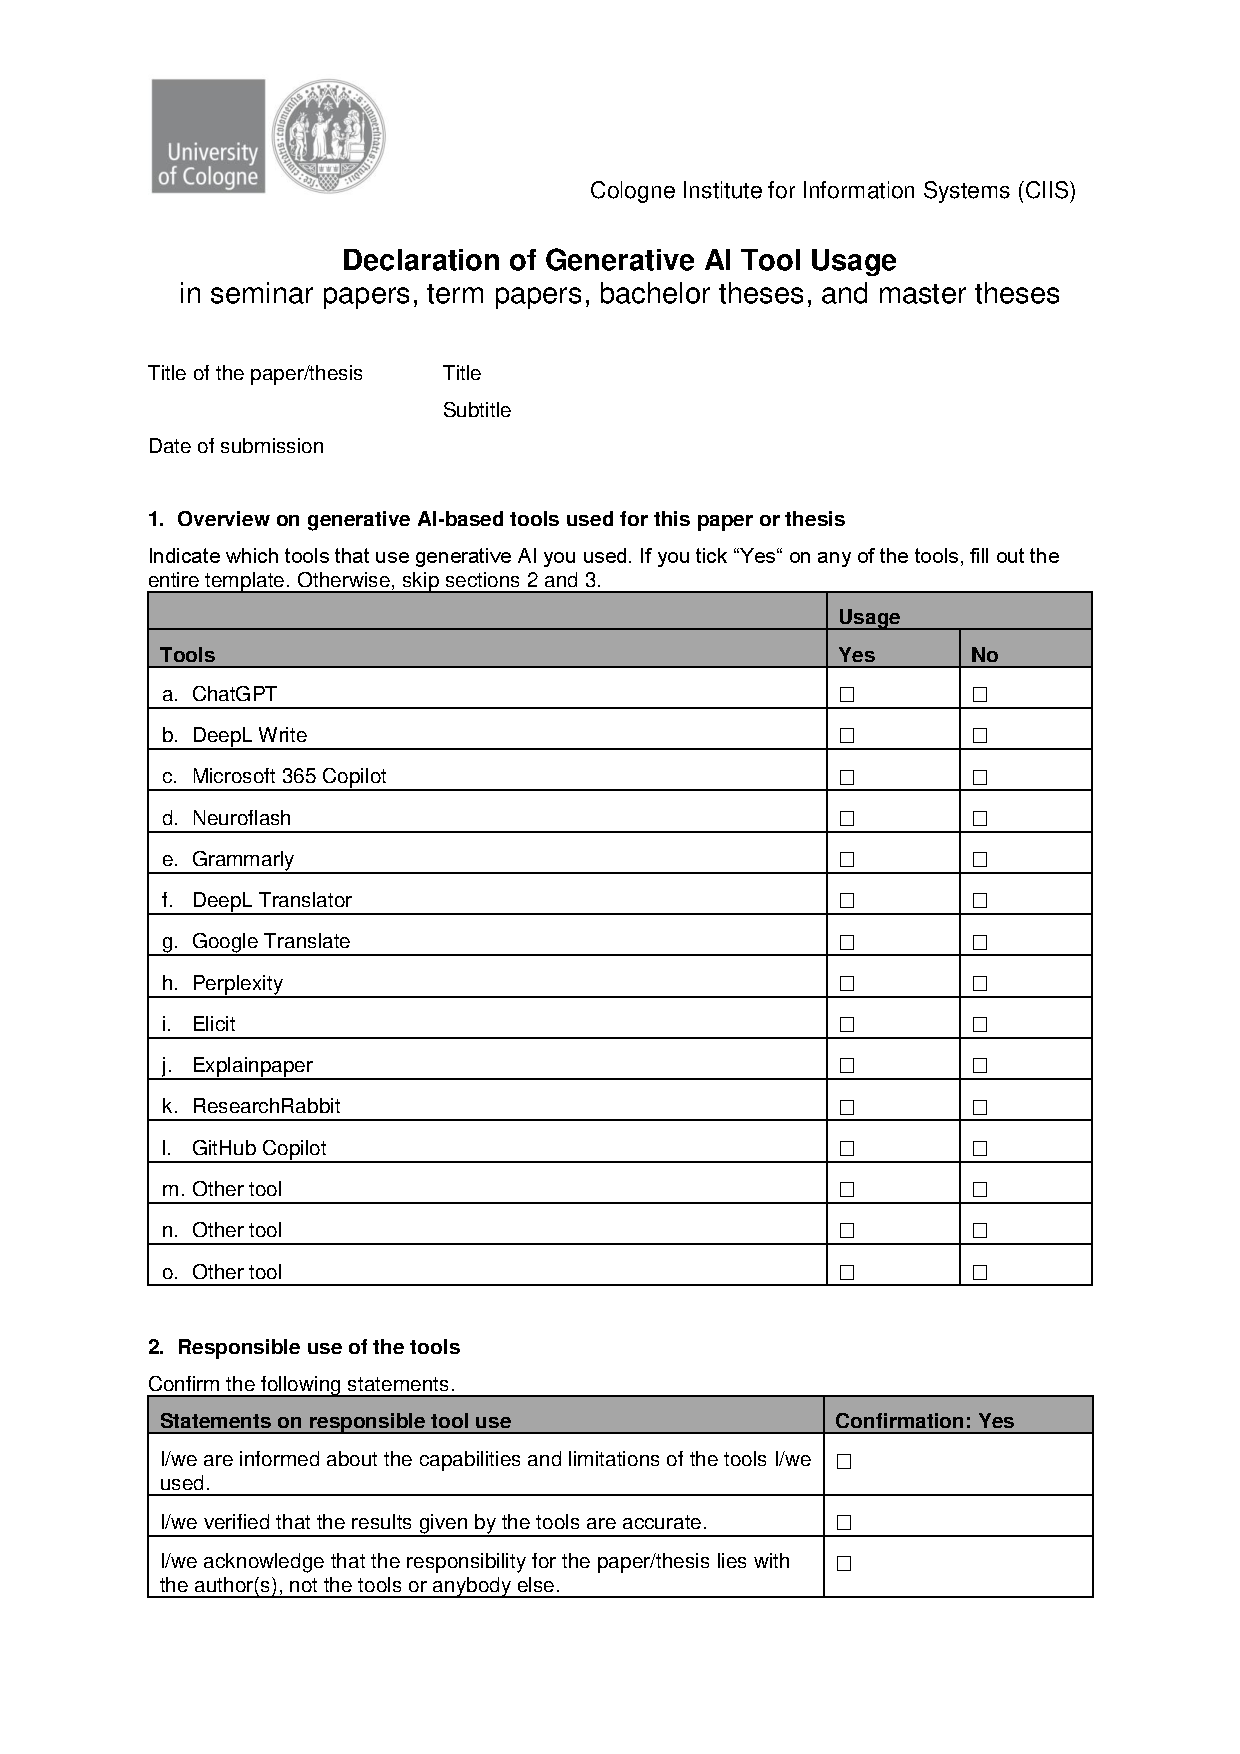
\includepdf[
  pages=1,
  width=\textwidth,
  offset=0.75cm 0cm,
  frame,
  pagecommand={
    \section*{Declaration of Generative AI Tool Usage}
    \addcontentsline{toc}{section}{Declaration of Generative AI Tool Usage}
  }
]{appendix/declaration-gen-ai-usage.pdf}
\includepdf[
  pages=2-,
  width=\textwidth,
  offset=0.75cm 0cm,
  frame,
  pagecommand={}
]{appendix/declaration-gen-ai-usage.pdf}

\end{document}